\documentclass[11pt]{article}
\usepackage{working-paper}
\usepackage{amsmath,amsthm}
\usepackage{graphicx,booktabs,longtable,array}
\usepackage{listings}
\usepackage{xurl}
\usepackage{enumitem}

\newtheorem{proposition}{Proposition}
\lstset{basicstyle=\small\ttfamily,breaklines=true,columns=fullflexible,keepspaces=true}
\setlength{\emergencystretch}{2em}
\graphicspath{{generated/}}
\newcommand{\CenHgbIpfBrier}{0.5703}
\newcommand{\CenHgbIpfNll}{1.1702}
\newcommand{\CenHgbIpfRank}{93.4}
\newcommand{\CenHgbKlSoftBrier}{0.5481}
\newcommand{\CenHgbKlSoftNll}{1.1279}
\newcommand{\CenHgbKlSoftRank}{96.2}
\newcommand{\CenHgbKlWeakBrier}{0.5758}
\newcommand{\CenHgbKlWeakNll}{1.1659}
\newcommand{\CenHgbKlWeakRank}{100.0}
\newcommand{\CenHgbOrigBrier}{0.7101}
\newcommand{\CenHgbOrigNll}{1.5539}
\newcommand{\CenHgbOrigRank}{100.0}
\newcommand{\CenHgbTempIpfBrier}{0.5324}
\newcommand{\CenHgbTempIpfNll}{1.0141}
\newcommand{\CenHgbTempIpfRank}{93.1}
\newcommand{\CenHgbTempKlSoftBrier}{0.5302}
\newcommand{\CenHgbTempKlSoftNll}{1.0237}
\newcommand{\CenHgbTempKlSoftRank}{97.0}
\newcommand{\CenIpfBrier}{0.5810}
\newcommand{\CenIpfMaxViol}{0.474}
\newcommand{\CenIpfNll}{1.2677}
\newcommand{\CenIpfRank}{93.7}
\newcommand{\CenKlSoftBrier}{0.5671}
\newcommand{\CenKlSoftMaxViol}{0.482}
\newcommand{\CenKlSoftNll}{1.2305}
\newcommand{\CenKlSoftRank}{96.6}
\newcommand{\CenKlWeakBrier}{0.5816}
\newcommand{\CenKlWeakMaxViol}{0.000}
\newcommand{\CenKlWeakNll}{1.1559}
\newcommand{\CenKlWeakRank}{100.0}
\newcommand{\CenLrIpfBrier}{0.5286}
\newcommand{\CenLrIpfNll}{1.0169}
\newcommand{\CenLrIpfRank}{93.9}
\newcommand{\CenLrKlSoftBrier}{0.5359}
\newcommand{\CenLrKlSoftNll}{1.0384}
\newcommand{\CenLrKlSoftRank}{98.0}
\newcommand{\CenLrKlWeakBrier}{0.5799}
\newcommand{\CenLrKlWeakNll}{1.1158}
\newcommand{\CenLrKlWeakRank}{100.0}
\newcommand{\CenLrOrigBrier}{0.6840}
\newcommand{\CenLrOrigNll}{1.3092}
\newcommand{\CenLrOrigRank}{100.0}
\newcommand{\CenLrTempIpfBrier}{0.5291}
\newcommand{\CenLrTempIpfNll}{1.0153}
\newcommand{\CenLrTempIpfRank}{93.8}
\newcommand{\CenLrTempKlSoftBrier}{0.5369}
\newcommand{\CenLrTempKlSoftNll}{1.0375}
\newcommand{\CenLrTempKlSoftRank}{98.0}
\newcommand{\CenMlpIpfBrier}{0.6453}
\newcommand{\CenMlpIpfNll}{1.5856}
\newcommand{\CenMlpIpfRank}{93.5}
\newcommand{\CenMlpKlSoftBrier}{0.6186}
\newcommand{\CenMlpKlSoftNll}{1.5043}
\newcommand{\CenMlpKlSoftRank}{95.5}
\newcommand{\CenMlpKlWeakBrier}{0.5885}
\newcommand{\CenMlpKlWeakNll}{1.2024}
\newcommand{\CenMlpKlWeakRank}{100.0}
\newcommand{\CenMlpOrigBrier}{0.7452}
\newcommand{\CenMlpOrigNll}{1.9837}
\newcommand{\CenMlpOrigRank}{100.0}
\newcommand{\CenMlpTempIpfBrier}{0.5733}
\newcommand{\CenMlpTempIpfNll}{1.1313}
\newcommand{\CenMlpTempIpfRank}{92.6}
\newcommand{\CenMlpTempKlSoftBrier}{0.5696}
\newcommand{\CenMlpTempKlSoftNll}{1.1204}
\newcommand{\CenMlpTempKlSoftRank}{96.7}
\newcommand{\CenOrigBrier}{0.7093}
\newcommand{\CenOrigMaxViol}{0.000}
\newcommand{\CenOrigNll}{1.6111}
\newcommand{\CenOrigRank}{100.0}
\newcommand{\CenTempIpfBrier}{0.5479}
\newcommand{\CenTempIpfMaxViol}{0.351}
\newcommand{\CenTempIpfNll}{1.0680}
\newcommand{\CenTempIpfRank}{92.8}
\newcommand{\CenTempKlSoftBrier}{0.5491}
\newcommand{\CenTempKlSoftMaxViol}{0.328}
\newcommand{\CenTempKlSoftNll}{1.0686}
\newcommand{\CenTempKlSoftRank}{97.1}
\newcommand{\CovEucAuroc}{0.8379}
\newcommand{\CovEucBrier}{0.4878}
\newcommand{\CovEucConv}{12.0}
\newcommand{\CovEucDBrier}{+20.9}
\newcommand{\CovEucDBrierHi}{+52.0}
\newcommand{\CovEucDBrierLo}{-4.6}
\newcommand{\CovEucDNll}{+64.3}
\newcommand{\CovEucDRank}{+9.18}
\newcommand{\CovEucMaxViol}{0.000}
\newcommand{\CovEucNll}{1.1132}
\newcommand{\CovEucRank}{100.0}
\newcommand{\CovIpfAuroc}{0.8404}
\newcommand{\CovIpfBrier}{0.5397}
\newcommand{\CovIpfConv}{100.0}
\newcommand{\CovIpfDBrier}{+0.0}
\newcommand{\CovIpfDBrierHi}{+0.0}
\newcommand{\CovIpfDBrierLo}{+0.0}
\newcommand{\CovIpfDNll}{+0.0}
\newcommand{\CovIpfDRank}{+0.00}
\newcommand{\CovIpfMaxViol}{0.635}
\newcommand{\CovIpfNll}{1.3007}
\newcommand{\CovIpfRank}{89.0}
\newcommand{\CovKlSoftAuroc}{0.8382}
\newcommand{\CovKlSoftBrier}{0.5274}
\newcommand{\CovKlSoftConv}{99.0}
\newcommand{\CovKlSoftDBrier}{+12.3}
\newcommand{\CovKlSoftDBrierHi}{+16.3}
\newcommand{\CovKlSoftDBrierLo}{+8.6}
\newcommand{\CovKlSoftDNll}{+56.7}
\newcommand{\CovKlSoftDRank}{+2.37}
\newcommand{\CovKlSoftMaxViol}{0.572}
\newcommand{\CovKlSoftNll}{1.2415}
\newcommand{\CovKlSoftRank}{91.4}
\newcommand{\CovKlWeakAuroc}{0.8199}
\newcommand{\CovKlWeakBrier}{0.5565}
\newcommand{\CovKlWeakConv}{97.4}
\newcommand{\CovKlWeakDBrier}{-17.3}
\newcommand{\CovKlWeakDBrierHi}{-5.3}
\newcommand{\CovKlWeakDBrierLo}{-30.4}
\newcommand{\CovKlWeakDNll}{+92.5}
\newcommand{\CovKlWeakDRank}{+10.96}
\newcommand{\CovKlWeakMaxViol}{0.000}
\newcommand{\CovKlWeakNll}{1.2038}
\newcommand{\CovKlWeakRank}{100.0}
\newcommand{\CovOrigAuroc}{0.8255}
\newcommand{\CovOrigBrier}{0.7419}
\newcommand{\CovOrigConv}{100.0}
\newcommand{\CovOrigDBrier}{-202.2}
\newcommand{\CovOrigDBrierHi}{-175.6}
\newcommand{\CovOrigDBrierLo}{-228.8}
\newcommand{\CovOrigDNll}{-1223.7}
\newcommand{\CovOrigDRank}{+11.00}
\newcommand{\CovOrigMaxViol}{0.000}
\newcommand{\CovOrigNll}{2.5244}
\newcommand{\CovOrigRank}{100.0}
\newcommand{\CovOverIpfBrier}{0.5893}
\newcommand{\CovOverIpfNll}{1.5261}
\newcommand{\CovOverIpfRank}{87.9}
\newcommand{\CovOverKlSoftBrier}{0.5617}
\newcommand{\CovOverKlSoftNll}{1.4336}
\newcommand{\CovOverKlSoftRank}{89.9}
\newcommand{\CovOverKlWeakBrier}{0.5744}
\newcommand{\CovOverKlWeakNll}{1.3187}
\newcommand{\CovOverKlWeakRank}{100.0}
\newcommand{\CovOverTempIpfBrier}{0.5316}
\newcommand{\CovOverTempIpfNll}{1.1006}
\newcommand{\CovOverTempIpfRank}{84.9}
\newcommand{\CovOverTempKlSoftBrier}{0.5187}
\newcommand{\CovOverTempKlSoftNll}{1.0805}
\newcommand{\CovOverTempKlSoftRank}{90.1}
\newcommand{\CovTempIpfAuroc}{0.8410}
\newcommand{\CovTempIpfBrier}{0.5033}
\newcommand{\CovTempIpfConv}{100.0}
\newcommand{\CovTempIpfDBrier}{+36.4}
\newcommand{\CovTempIpfDBrierHi}{+42.7}
\newcommand{\CovTempIpfDBrierLo}{+30.0}
\newcommand{\CovTempIpfDNll}{+173.6}
\newcommand{\CovTempIpfDRank}{-1.41}
\newcommand{\CovTempIpfMaxViol}{0.543}
\newcommand{\CovTempIpfNll}{1.1271}
\newcommand{\CovTempIpfRank}{87.6}
\newcommand{\CovTempKlSoftAuroc}{0.8399}
\newcommand{\CovTempKlSoftBrier}{0.4966}
\newcommand{\CovTempKlSoftConv}{97.9}
\newcommand{\CovTempKlSoftDBrier}{+39.8}
\newcommand{\CovTempKlSoftDBrierHi}{+47.5}
\newcommand{\CovTempKlSoftDBrierLo}{+32.4}
\newcommand{\CovTempKlSoftDNll}{+140.8}
\newcommand{\CovTempKlSoftDRank}{+2.41}
\newcommand{\CovTempKlSoftMaxViol}{0.423}
\newcommand{\CovTempKlSoftNll}{1.1482}
\newcommand{\CovTempKlSoftRank}{91.7}
\newcommand{\DigitsEucConvPct}{0}
\newcommand{\DigitsKlSoftConvPct}{100}
\newcommand{\DigitsKlWeakConvPct}{86}
\newcommand{\DigitsTempKlSoftConvPct}{100}
\newcommand{\LabEucAuroc}{0.9976}
\newcommand{\LabEucBrier}{0.0391}
\newcommand{\LabEucConv}{17.1}
\newcommand{\LabEucDBrier}{-5.5}
\newcommand{\LabEucDBrierHi}{-2.0}
\newcommand{\LabEucDBrierLo}{-9.7}
\newcommand{\LabEucDNll}{-28.7}
\newcommand{\LabEucDRank}{+2.49}
\newcommand{\LabEucMaxViol}{0.000}
\newcommand{\LabEucNll}{0.1010}
\newcommand{\LabEucRank}{100.0}
\newcommand{\LabIpfAuroc}{0.9220}
\newcommand{\LabIpfBrier}{0.2458}
\newcommand{\LabIpfConv}{94.6}
\newcommand{\LabIpfDBrier}{+0.0}
\newcommand{\LabIpfDBrierHi}{+0.0}
\newcommand{\LabIpfDBrierLo}{+0.0}
\newcommand{\LabIpfDNll}{+0.0}
\newcommand{\LabIpfDRank}{+0.00}
\newcommand{\LabIpfMaxViol}{0.459}
\newcommand{\LabIpfNll}{0.5221}
\newcommand{\LabIpfRank}{95.6}
\newcommand{\LabKlSoftAuroc}{0.9228}
\newcommand{\LabKlSoftBrier}{0.2351}
\newcommand{\LabKlSoftConv}{97.1}
\newcommand{\LabKlSoftDBrier}{-1.2}
\newcommand{\LabKlSoftDBrierHi}{+0.9}
\newcommand{\LabKlSoftDBrierLo}{-3.2}
\newcommand{\LabKlSoftDNll}{+1.7}
\newcommand{\LabKlSoftDRank}{+2.21}
\newcommand{\LabKlSoftMaxViol}{0.376}
\newcommand{\LabKlSoftNll}{0.4945}
\newcommand{\LabKlSoftRank}{97.9}
\newcommand{\LabKlWeakAuroc}{0.9179}
\newcommand{\LabKlWeakBrier}{0.3053}
\newcommand{\LabKlWeakConv}{97.9}
\newcommand{\LabKlWeakDBrier}{-70.3}
\newcommand{\LabKlWeakDBrierHi}{-55.9}
\newcommand{\LabKlWeakDBrierLo}{-84.4}
\newcommand{\LabKlWeakDNll}{-112.8}
\newcommand{\LabKlWeakDRank}{+4.38}
\newcommand{\LabKlWeakMaxViol}{0.000}
\newcommand{\LabKlWeakNll}{0.6143}
\newcommand{\LabKlWeakRank}{100.0}
\newcommand{\LabOrigAuroc}{0.9210}
\newcommand{\LabOrigBrier}{0.3290}
\newcommand{\LabOrigConv}{100.0}
\newcommand{\LabOrigDBrier}{-100.1}
\newcommand{\LabOrigDBrierHi}{-87.1}
\newcommand{\LabOrigDBrierLo}{-112.5}
\newcommand{\LabOrigDNll}{-229.0}
\newcommand{\LabOrigDRank}{+4.36}
\newcommand{\LabOrigMaxViol}{0.000}
\newcommand{\LabOrigNll}{0.7143}
\newcommand{\LabOrigRank}{100.0}
\newcommand{\LabTempIpfAuroc}{0.9157}
\newcommand{\LabTempIpfBrier}{0.2438}
\newcommand{\LabTempIpfConv}{87.5}
\newcommand{\LabTempIpfDBrier}{+19.5}
\newcommand{\LabTempIpfDBrierHi}{+22.8}
\newcommand{\LabTempIpfDBrierLo}{+16.3}
\newcommand{\LabTempIpfDNll}{+105.5}
\newcommand{\LabTempIpfDRank}{-1.88}
\newcommand{\LabTempIpfMaxViol}{0.427}
\newcommand{\LabTempIpfNll}{0.4560}
\newcommand{\LabTempIpfRank}{93.3}
\newcommand{\LabTempKlSoftAuroc}{0.9226}
\newcommand{\LabTempKlSoftBrier}{0.2220}
\newcommand{\LabTempKlSoftConv}{99.2}
\newcommand{\LabTempKlSoftDBrier}{+13.1}
\newcommand{\LabTempKlSoftDBrierHi}{+17.1}
\newcommand{\LabTempKlSoftDBrierLo}{+9.4}
\newcommand{\LabTempKlSoftDNll}{+87.2}
\newcommand{\LabTempKlSoftDRank}{+2.06}
\newcommand{\LabTempKlSoftMaxViol}{0.310}
\newcommand{\LabTempKlSoftNll}{0.4153}
\newcommand{\LabTempKlSoftRank}{97.6}
\newcommand{\NumDatasets}{6}
\newcommand{\NumModels}{4}
\newcommand{\NumRealSeeds}{10}
\newcommand{\NumSynthSeeds}{20}
\newcommand{\NumTotalRealRuns}{3,024}
\newcommand{\RealEucConvPct}{14.8}
\newcommand{\RealKlSoftConvPct}{97.9}
\newcommand{\RealKlWeakConvPct}{97.7}
\newcommand{\RealTempKlSoftConvPct}{98.6}
\newcommand{\SoftLam}{2}
\newcommand{\SynCovEucBrier}{--}
\newcommand{\SynCovEucRank}{--}
\newcommand{\SynCovEucRmse}{--}
\newcommand{\SynCovIpfBrier}{0.5249}
\newcommand{\SynCovIpfRank}{93.0}
\newcommand{\SynCovIpfRmse}{0.1069}
\newcommand{\SynCovKlSoftBrier}{0.5002}
\newcommand{\SynCovKlSoftRank}{95.9}
\newcommand{\SynCovKlSoftRmse}{0.0587}
\newcommand{\SynCovKlWeakBrier}{0.4975}
\newcommand{\SynCovKlWeakRank}{100.0}
\newcommand{\SynCovKlWeakRmse}{0.0529}
\newcommand{\SynCovOrigBrier}{0.6361}
\newcommand{\SynCovOrigRank}{100.0}
\newcommand{\SynCovOrigRmse}{0.2160}
\newcommand{\SynOverEucBrier}{--}
\newcommand{\SynOverEucRank}{--}
\newcommand{\SynOverEucRmse}{--}
\newcommand{\SynOverIpfBrier}{0.4227}
\newcommand{\SynOverIpfRank}{95.0}
\newcommand{\SynOverIpfRmse}{0.1253}
\newcommand{\SynOverKlSoftBrier}{0.4222}
\newcommand{\SynOverKlSoftRank}{94.2}
\newcommand{\SynOverKlSoftRmse}{0.1221}
\newcommand{\SynOverKlWeakBrier}{0.4157}
\newcommand{\SynOverKlWeakRank}{100.0}
\newcommand{\SynOverKlWeakRmse}{0.1169}
\newcommand{\SynOverOrigBrier}{0.5421}
\newcommand{\SynOverOrigRank}{100.0}
\newcommand{\SynOverOrigRmse}{0.2314}
\newcommand{\SynPureEucBrier}{--}
\newcommand{\SynPureEucRank}{--}
\newcommand{\SynPureEucRmse}{--}
\newcommand{\SynPureIpfBrier}{0.3741}
\newcommand{\SynPureIpfRank}{94.5}
\newcommand{\SynPureIpfRmse}{0.0000}
\newcommand{\SynPureKlSoftBrier}{0.3826}
\newcommand{\SynPureKlSoftRank}{95.7}
\newcommand{\SynPureKlSoftRmse}{0.0541}
\newcommand{\SynPureKlWeakBrier}{0.4216}
\newcommand{\SynPureKlWeakRank}{100.0}
\newcommand{\SynPureKlWeakRmse}{0.1261}
\newcommand{\SynPureOrigBrier}{0.4698}
\newcommand{\SynPureOrigRank}{100.0}
\newcommand{\SynPureOrigRmse}{0.1744}
\newcommand{\TieKlDropPct}{8.3}
\newcommand{\TieStableConvPct}{100}


\title{When Marginal Calibration Scrambles Ranks:\\
Weak-Order KL Calibration for Multiclass Probabilities\thanks{Software and replication materials: \url{https://github.com/finite-sample/rank-preserving-calibration} (v0.12.0).}}

\author{Gaurav Sood}
\date{}

\begin{document}

\maketitle

\begin{abstract}
Matching predicted class probabilities to known population totals is routine in survey post-calibration and shifted-domain deployment. For binary outcomes, the standard intercept shift (logit correction) is strictly monotone and preserves every individual's relative rank. For three or more classes, however, multinomial intercept correction---equivalently Iterative Proportional Fitting (IPF)---depends on an instance-specific normalizing denominator and can reverse within-class rankings \citep{mitchell2025}. We formalize when those reversals occur, prove that IPF preserves every pairwise odds ratio and is Bayes-optimal under pure label shift---making exact Bayes optimality, exact marginal matching, and within-class rank preservation mutually incompatible---and formulate exact weak-order Kullback--Leibler (KL) calibration on the transportation polytope. Using monotone block-boundary variables, our conic formulation handles tied discrete scores without arbitrary tie-breaking, reducing KL divergence by \TieKlDropPct\% over row-order tie constraints while explaining why KL geometry succeeds where Euclidean Dykstra projection fails (\RealKlSoftConvPct\%--\RealTempKlSoftConvPct\% versus \RealEucConvPct\% solver convergence). Across an exact-posterior synthetic study and \NumTotalRealRuns{} real-data runs spanning \NumDatasets{} multiclass datasets ($J=3$ to $10$, including a US Census CPS subpopulation shift), \NumModels{} model families, and two shift regimes, strict weak-order preservation carries a real Brier cost under pure label shift (\LabKlWeakDBrier{}$\times 10^{-3}$ versus IPF), whereas soft KL calibration ($\lambda=\SoftLam$) recovers most rank inversions at negligible cost (\LabKlSoftDBrier{}$\times 10^{-3}$). Under covariate shift and overconfident nonlinear models, soft KL calibration and anchor-reference-decoupled temperature-plus-KL calibration simultaneously improve held-out Brier score (\CovKlSoftDBrier{} and \CovTempKlSoftDBrier{}$\times 10^{-3}$ over IPF) and preserve within-class rankings while matching target totals exactly.
\end{abstract}

\section{Introduction}

In survey statistics, ecological inference, and shifted-domain classification, a practitioner often holds individual-level predicted class probabilities $P \in \mathbb{R}_+^{N \times J}$ alongside known aggregate class totals $T \in \mathbb{R}_+^J$ with $\sum_{j=1}^J T_j = N$. Examples include calibrating multilevel regression and poststratification (MRP) vote-share predictions for multi-candidate elections to official turnout totals, adjusting predicted demographic probabilities to Census counts, and adapting a deployed classifier to a target population with different class prevalence \citep{saerens2002,lipton2018}.

When the outcome is binary ($J=2$), matching the aggregate total by a constant intercept shift on the log-odds scale, $Q_{i1} = \operatorname{logistic}(\operatorname{logit}(P_{i1}) + \delta)$, is strictly increasing in $P_{i1}$. It simultaneously matches the target total, minimizes Kullback--Leibler (KL) divergence from $P$, yields the exact Bayes posterior under pure label shift, and preserves the exact ranking of all $N$ units.

As \citet{mitchell2025} observed, that harmony breaks down as soon as $J \ge 3$. The multinomial intercept shift---solved by Iterative Proportional Fitting (IPF) or Sinkhorn scaling \citep{deming1940,sinkhorn1967,ireland1968}---updates each row via
\begin{equation}
Q_{ij} = \frac{b_j P_{ij}}{\sum_{k=1}^J b_k P_{ik}},
\label{eq:ipf}
\end{equation}
where $b_1,\dots,b_J > 0$ are chosen so that $\sum_{i=1}^N Q_{ij} = T_j$. Because the denominator $\sum_k b_k P_{ik}$ varies across rows $i$, two units with $P_{i_1 j} > P_{i_2 j}$ can invert to $Q_{i_1 j} < Q_{i_2 j}$. Consider a concrete three-class example with two units and multipliers $b = (1, 100, 1)$:
\[
P_{1,\cdot} = (0.51,\, 0.48,\, 0.01), \qquad P_{2,\cdot} = (0.49,\, 0.02,\, 0.49).
\]
After scaling, $Q_{11} = 0.51 / 48.52 \approx 0.0105$ while $Q_{21} = 0.49 / 3.00 \approx 0.1633$: unit 1 had the higher initial probability for class 1, yet ends up more than fifteen times lower than unit 2.

That example immediately raises a substantive question that existing calibration work leaves unanswered: \emph{is this rank reversal a defect to fix, or a feature of Bayes' rule?} Under pure label shift---where class-conditional feature distributions $P(X \mid Y)$ are unchanged and only class priors move---unit 1's large probability on class 2 ($0.48$) means a 100-fold surge in class 2 makes unit 1 almost certainly class 2, legitimately pushing its class-1 probability below unit 2's. In that setting, forcing strict rank preservation fights the Bayes posterior. By contrast, when the base classifier is overconfident, when $P(X \mid Y)$ also shifts across subpopulations (covariate shift), or when institutional rules prohibit post-hoc marginal calibration from demoting higher-scoring units within a class (e.g., triage queues, risk scoring, or fairness-constrained prioritization), wild denominator-driven inversions are harmful.

Prior work on multiclass post-hoc calibration addresses different targets. Temperature scaling \citep{guo2017}, Dirichlet calibration \citep{kull2019}, Meta-Cal \citep{ma2021metacal}, and intra-order-preserving neural maps \citep{rahimi2020} optimize held-out proper scores or preserve \emph{within-instance} top-$k$ class orderings ($P_{i j_1} \le P_{i j_2} \implies Q_{i j_1} \le Q_{i j_2}$). None simultaneously enforces exact \emph{column marginal totals} $\sum_i Q_{ij} = T_j$ and \emph{within-class across-instance} ordering ($P_{i_1 j} < P_{i_2 j} \implies Q_{i_1 j} \le Q_{i_2 j}$). Conversely, label-shift estimators \citep{saerens2002,lipton2018} match marginals via~\eqref{eq:ipf} without controlling within-class reversals.

This paper makes four contributions:
\begin{enumerate}[leftmargin=*,itemsep=2pt]
\item \textbf{Formalizing the tradeoff:} We characterize exactly when IPF reverses within-class ranks, prove that IPF preserves all pairwise odds ratios, and establish the three-way impossibility among exact Bayes optimality under pure label shift, exact marginal matching, and strict within-class rank preservation for $J \ge 3$ (Proposition~1).
\item \textbf{Exact weak-order KL conic formulation:} We replace arbitrary row-order tie constraints with monotone block-boundary variables (Proposition~2), derive the Bregman KKT conditions showing why KL geometry stays multiplicative on the open simplex while Euclidean projection clips probabilities and stalls (Proposition~3), and formulate the soft $\lambda$-Pareto frontier with anchor-reference decoupling (Proposition~4).
\item \textbf{Broad, honest empirical evidence:} Across an exact-posterior synthetic study (\NumSynthSeeds{} seeds) and \NumTotalRealRuns{} real-data runs spanning \NumDatasets{} datasets ($J=3$ to $10$, including a US Census CPS subpopulation shift), \NumModels{} model families, and both pure label shift and covariate shift, we compare against true IPF, temperature scaling plus IPF, and Euclidean projection.
\item \textbf{Open-source software:} All exact conic solvers (\texttt{ties="weak"} default), diagnostics, and replication scripts are implemented and tested in \texttt{rank-preserving-calibration} v0.12.0.
\end{enumerate}

\section{When Marginal Calibration Reverses Ranks}

Let $P \in (0,1)^{N \times J}$ be a matrix of predicted probabilities whose rows lie on the probability simplex $\Delta^{J-1} = \{q \in \mathbb{R}_+^J : \sum_{j=1}^J q_j = 1\}$, and let $T \in \mathbb{R}_{++}^J$ be target column totals with $\sum_{j=1}^J T_j = N$. Define the transportation polytope
\[
\mathcal{C}(T) = \left\{ Q \in \mathbb{R}_+^{N \times J} : Q\mathbf{1}_J = \mathbf{1}_N,\; Q^\top \mathbf{1}_N = T \right\}.
\]
The classical minimum-KL marginal adjustment solves $\min_{Q \in \mathcal{C}(T)} \operatorname{KL}(Q \| P)$, where $\operatorname{KL}(Q \| P) = \sum_{i,j} Q_{ij} \log(Q_{ij}/P_{ij})$. By strict convexity, this problem has a unique solution of the multiplicative form~\eqref{eq:ipf}, which IPF (Sinkhorn scaling) computes \citep{ireland1968}.

Within class $j$, we say $Q$ preserves the \emph{weak order} of an anchor matrix $A \in \mathbb{R}^{N \times J}$ (default $A = P$) if
\begin{equation}
A_{i_1 j} < A_{i_2 j} \;\Longrightarrow\; Q_{i_1 j} \le Q_{i_2 j}
\qquad \text{for all } i_1, i_2 \in \{1,\dots,N\},\; j \in \{1,\dots,J\}.
\label{eq:weak_order}
\end{equation}
Tied anchor scores ($A_{i_1 j} = A_{i_2 j}$) impose no relative constraint between $Q_{i_1 j}$ and $Q_{i_2 j}$. Notice the distinction from \citet{rahimi2020}, who constrain the ordering \emph{across classes within a row} ($j_1$ vs.\ $j_2$ for fixed $i$); here we constrain the ordering \emph{across units within a column} ($i_1$ vs.\ $i_2$ for fixed $j$).

\begin{proposition}[IPF Rank Reversals, Odds-Ratio Invariance, and Pure-Label-Shift Impossibility]
\label{prop:ipf}
Let $Q^{\mathrm{IPF}} \in \mathcal{C}(T)$ be the unique solution to~\eqref{eq:ipf} with positive multipliers $b_1,\dots,b_J > 0$.
\begin{enumerate}[label=(\alph*),leftmargin=*,itemsep=2pt]
\item \textbf{Binary preservation:} If $J=2$, $Q^{\mathrm{IPF}}$ preserves the strict within-class ordering of $P$ in every column.
\item \textbf{Pairwise odds-ratio invariance:} For any $J \ge 2$ and any pair of classes $j, k$,
\[
\frac{P_{i_1 j}}{P_{i_1 k}} < \frac{P_{i_2 j}}{P_{i_2 k}}
\;\Longleftrightarrow\;
\frac{Q^{\mathrm{IPF}}_{i_1 j}}{Q^{\mathrm{IPF}}_{i_1 k}} < \frac{Q^{\mathrm{IPF}}_{i_2 j}}{Q^{\mathrm{IPF}}_{i_2 k}}.
\]
\item \textbf{Exact reversal condition ($J \ge 3$):} A pair with $P_{i_1 j} > P_{i_2 j}$ inverts to $Q^{\mathrm{IPF}}_{i_1 j} < Q^{\mathrm{IPF}}_{i_2 j}$ if and only if
\[
\frac{\sum_{k=1}^J b_k P_{i_1 k}}{\sum_{k=1}^J b_k P_{i_2 k}} > \frac{P_{i_1 j}}{P_{i_2 j}},
\]
which requires at least one third class $k \ne j$ with $b_k \ne b_j$ and $P_{i_1 k} \ne P_{i_2 k}$.
\item \textbf{Impossibility under pure label shift:} When $P_{ij} = P_{\mathrm{src}}(Y=j \mid X_i)$ is the exact source Bayes posterior and the target domain differs only by class priors ($P_{\mathrm{tgt}}(X \mid Y) = P_{\mathrm{src}}(X \mid Y)$) with $T_j = \sum_i P_{\mathrm{tgt}}(Y=j \mid X_i)$, $Q^{\mathrm{IPF}}$ equals the exact target Bayes posterior. Consequently, for $J \ge 3$, exact Bayes optimality under pure label shift, exact marginal matching, and strict within-class weak-order preservation~\eqref{eq:weak_order} are mutually incompatible whenever condition~(c) holds.
\end{enumerate}
\end{proposition}

The proof is in Appendix~\ref{app:proofs}. Proposition~\ref{prop:ipf} clarifies the entire conceptual debate. IPF does not scramble pairwise comparisons between two specific classes: the odds of class $j$ versus class $k$ remain strictly ordered across all units. Reversals enter solely through third-class denominator shifts. When pure label shift holds and $P$ is already calibrated, those denominator shifts are Bayes-optimal, so strict rank preservation must sacrifice posterior accuracy. When $P$ is overconfident or when $P(X \mid Y)$ shifts across domains, however, extreme entries in $P$ interact with large multipliers $b_k$ to amplify denominator swings—creating both severe rank reversals and inflated probability error.

\section{Exact Weak-Order KL Calibration}

To enforce or regularize~\eqref{eq:weak_order} on the transportation polytope $\mathcal{C}(T)$, we solve a convex Bregman projection onto $\mathcal{C}(T)$ subject to exact weak-order constraints. Two design choices turn out to be decisive: how tied anchor scores are represented, and whether the divergence is KL or Euclidean.

\subsection{Exact Weak-Order Constraints via Block Boundaries}

A naive way to enforce isotonicity in column $j$ is to sort $A_{\cdot j}$ stably (breaking ties by row index) into a permutation $\pi_j$ and require $Q_{\pi_j(1),j} \le \cdots \le Q_{\pi_j(N),j}$. When scores are continuous and distinct, this is exact. On real classifiers such as random forests, bagged trees, or rounded survey probabilities, however, hundreds of rows share identical scores. Stable sorting then imposes hundreds of arbitrary inequalities between tied rows, making the solution depend on row ordering, inflating divergence, and triggering numerical failures when a solver struggles with redundant active faces.

Instead, partition $\{1,\dots,N\}$ in column $j$ into $K_j$ strictly ordered tie blocks $B_{j,1} \prec \cdots \prec B_{j,K_j}$, so that $i, i' \in B_{j,k} \iff A_{ij} = A_{i'j}$ and $i \in B_{j,k},\, i' \in B_{j,k'}$ with $k < k' \iff A_{ij} < A_{i'j}$.

\begin{proposition}[Exact Weak-Order Block-Boundary Representation]
\label{prop:ties}
A matrix $Q \in \mathbb{R}^{N \times J}$ satisfies the weak-order condition~\eqref{eq:weak_order} if and only if for each column $j$ with $K_j \ge 2$ there exist boundary scalars $u_{j,1} \le u_{j,2} \le \cdots \le u_{j,K_j - 1}$ such that
\begin{equation}
Q_{ij} \le u_{j,k} \quad (\forall i \in B_{j,k},\; k < K_j),
\qquad
u_{j,k-1} \le Q_{ij} \quad (\forall i \in B_{j,k},\; k > 1).
\label{eq:boundaries}
\end{equation}
This representation uses at most $2N + K_j - 2 = O(N)$ linear inequalities per column, is invariant to arbitrary row permutations, and yields a strictly convex feasible set $\mathcal{W}(A) \subseteq \mathbb{R}^{N \times J}$ containing the stable-sort cone $\mathcal{S}(A)$. Consequently, for any strictly convex divergence $D_\phi(\cdot, R)$,
\[
\min_{Q \in \mathcal{C}(T) \cap \mathcal{W}(A)} D_\phi(Q, R) \;\le\; \min_{Q \in \mathcal{C}(T) \cap \mathcal{S}(A)} D_\phi(Q, R),
\]
with strict inequality whenever any arbitrary intra-tie constraint is active at the stable-sort optimum. Moreover, $\mathcal{C}(T) \cap \mathcal{W}(A)$ is always nonempty since the constant-column matrix $Q_{ij} = T_j/N$ is feasible.
\end{proposition}

\subsection{Bregman KKT Geometry: Why KL Succeeds Where Euclidean Fails}

Let $D_\phi(Q, R) = \sum_{i,j} [\phi(Q_{ij}) - \phi(R_{ij}) - \phi'(R_{ij})(Q_{ij} - R_{ij})]$ be the separable Bregman divergence generated by a strictly convex function $\phi$, and consider the soft-penalized calibration problem
\begin{equation}
\min_{Q \in \mathcal{C}(T),\; u,\; v \ge 0} \; D_\phi(Q, R) + \lambda \sum_{r} v_r,
\label{eq:soft}
\end{equation}
where $v_r \ge 0$ are hinge slacks relaxing the weak-order inequalities~\eqref{eq:boundaries} (or adjacent inequalities when $K_j = N$) and $\lambda \ge 0$ controls the penalty weight.

\begin{proposition}[Bregman KKT Structure]
\label{prop:bregman}
At any interior optimum $Q^\star$ of~\eqref{eq:soft}, there exist row multipliers $\nu_i$, column multipliers $\mu_j$, and rank-constraint multipliers $\gamma_{ij}$ (bounded in magnitude by $\lambda$ per active inequality) such that
\[
\phi'(Q^\star_{ij}) = \phi'(R_{ij}) - \nu_i - \mu_j - \gamma_{ij}.
\]
In particular:
\begin{enumerate}[label=(\alph*),leftmargin=*,itemsep=2pt]
\item \textbf{KL divergence} ($\phi(x) = x\log x - x$, $\phi'(x) = \log x$):
\[
Q^\star_{ij} = R_{ij}\exp(-\nu_i - \mu_j - \gamma_{ij}).
\]
Updates are multiplicative, remain strictly positive whenever $R_{ij} > 0$, preserve zeros ($R_{ij}=0 \implies Q^\star_{ij}=0$), and recover IPF~\eqref{eq:ipf} exactly at $\lambda = 0$ (where $\gamma_{ij} = 0$).
\item \textbf{Euclidean distance} ($\phi(x) = \tfrac{1}{2}x^2$, $\phi'(x) = x$):
\[
Q^\star_{ij} = \max\!\left(0,\; R_{ij} - \nu_i - \mu_j - \gamma_{ij}\right).
\]
Updates are additive and clip small probabilities onto the simplex boundary, distorting log-odds and creating slow alternating-projection convergence under Dykstra's method \citep{dykstra1983,bauschke1994}.
\end{enumerate}
\end{proposition}

\subsection{Soft \texorpdfstring{$\lambda$}{lambda}-Pareto Frontier and Anchor-Reference Decoupling}

Problem~\eqref{eq:soft} with $\phi(x) = x\log x - x$ separates two roles that need not use the same matrix: the \emph{KL reference} $R$ from which divergence is measured, and the \emph{ranking anchor} $A$ whose weak order is preserved. When a source validation split is available, one can temperature-scale $P$ to obtain $R = P_{\mathrm{temp}}$ (removing source overconfidence) while keeping $A = P$ as the anchor whose original rankings are respected.

\begin{proposition}[Exact Conic Solve and Pareto Monotonicity]
\label{prop:pareto}
For any $R \in \mathbb{R}_+^{N \times J}$, anchor $A$, targets $T$, and $\lambda \ge 0$, problem~\eqref{eq:soft} under KL divergence is an exponential-cone program with $O(NJ)$ variables and cones. Letting $Q^\star(\lambda)$ denote its unique minimizer and $V_A(Q) = \min_{u,v \ge 0} \sum_r v_r$ the optimal hinge violation:
\begin{enumerate}[label=(\alph*),leftmargin=*,itemsep=2pt]
\item $V_A(Q^\star(\lambda))$ is non-increasing in $\lambda$ and $\operatorname{KL}(Q^\star(\lambda) \| R)$ is non-decreasing in $\lambda$.
\item $\lambda = 0$ recovers IPF applied to $R$, and $\lambda \to \infty$ (or solving~\eqref{eq:boundaries} directly with $v \equiv 0$) yields the exact strict weak-order KL projection.
\end{enumerate}
\end{proposition}

In \texttt{rank-preserving-calibration} v0.12.0, both the direct strict weak-order problem ($v \equiv 0$) and the soft problem~\eqref{eq:soft} are solved to interior-point accuracy via Clarabel \citep{goulart2024clarabel}, avoiding the stalling of alternating Bregman projections \citep{bauschke2000} and Euclidean Dykstra \citep{dykstra1983,duchi2008,condat2016}. Appendix~\ref{app:proofs} gives the sparse conic matrix construction.

\section{Evidence}

We test the theory and solvers across three empirical studies: (1) an exact-posterior synthetic benchmark where ground-truth target probabilities are known in closed form, (2) a broad real-data benchmark spanning \NumDatasets{} datasets, \NumModels{} model families, and two shift regimes (\NumTotalRealRuns{} total runs), and (3) a focused survey-style subpopulation calibration study on US Census Current Population Survey (CPS) data. All tables, figures, and inline statistics are generated directly from committed benchmark outputs.

\subsection{Exact-Posterior Synthetic Benchmark}

We simulate $N = 250$ observations from a three-class bivariate Gaussian mixture over \NumSynthSeeds{} seeds, shifting class priors from $(0.45, 0.35, 0.20)$ to $(0.15, 0.60, 0.25)$. Because class-conditional densities are known, we compute the exact target Bayes posterior $P_{\mathrm{true}}$ and compare three regimes: (i) \emph{pure label shift} with the exact calibrated source posterior $P_{\mathrm{src}}$ as input, (ii) \emph{overconfident label shift} where the input is sharpened to $P_{\mathrm{in}} \propto P_{\mathrm{src}}^{2.5}$ (mimicking overconfident neural networks and boosted trees), and (iii) \emph{covariate shift} where target class means also translate. We also round inputs to multiples of $0.05$ to measure the tie-handling gain of Proposition~\ref{prop:ties}.

\begin{table}[htbp]
\centering\scriptsize\setlength{\tabcolsep}{3.5pt}
\caption{Exact-posterior synthetic benchmark (3-class Gaussian mixture, $N=250$, \NumSynthSeeds{} seeds). Target totals equal exact expected target counts. Euclidean RPC (Dykstra, 1,500 iterations) achieved 0\% convergence (``--''); KL soft uses $\lambda=\SoftLam$.}
\label{tab:synthetic}
\begin{tabular}{llrrrrrrr}
\toprule
 &  & RMSE to truth & Brier & NLL & Rank rate & Max viol. & Col err & Conv. (\%) \\
\midrule
Label shift (calib.) & Original & 0.1744 & 0.4698 & 0.7931 & 1.0000 & 0.000 & 47.89 & 100 \\
 & IPF & 0.0000 & 0.3741 & 0.6483 & 0.9451 & 0.312 & $<0.01$ & 100 \\
 & Euclidean RPC & -- & -- & -- & -- & -- & -- & 0 \\
 & KL weak (strict) & 0.1261 & 0.4216 & 0.7328 & 1.0000 & 0.000 & $<0.01$ & 100 \\
 & KL soft & 0.0541 & 0.3826 & 0.6700 & 0.9572 & 0.255 & $<0.01$ & 100 \\
Label shift (overconf.) & Original & 0.2314 & 0.5421 & 1.1234 & 1.0000 & 0.000 & 46.06 & 100 \\
 & IPF & 0.1253 & 0.4227 & 0.8705 & 0.9504 & 0.594 & $<0.01$ & 100 \\
 & Euclidean RPC & -- & -- & -- & -- & -- & -- & 0 \\
 & KL weak (strict) & 0.1169 & 0.4157 & 0.8030 & 1.0000 & 0.000 & $<0.01$ & 100 \\
 & KL soft & 0.1221 & 0.4222 & 0.8590 & 0.9418 & 0.635 & $<0.01$ & 100 \\
Covariate shift & Original & 0.2160 & 0.6361 & 1.0829 & 1.0000 & 0.000 & 55.22 & 100 \\
 & IPF & 0.1069 & 0.5249 & 0.8888 & 0.9304 & 0.343 & $<0.01$ & 100 \\
 & Euclidean RPC & -- & -- & -- & -- & -- & -- & 0 \\
 & KL weak (strict) & 0.0529 & 0.4975 & 0.8337 & 1.0000 & 0.000 & $<0.01$ & 100 \\
 & KL soft & 0.0587 & 0.5002 & 0.8375 & 0.9587 & 0.242 & $<0.01$ & 100 \\
\bottomrule
\end{tabular}

\end{table}

\begin{figure}[htbp]
\centering
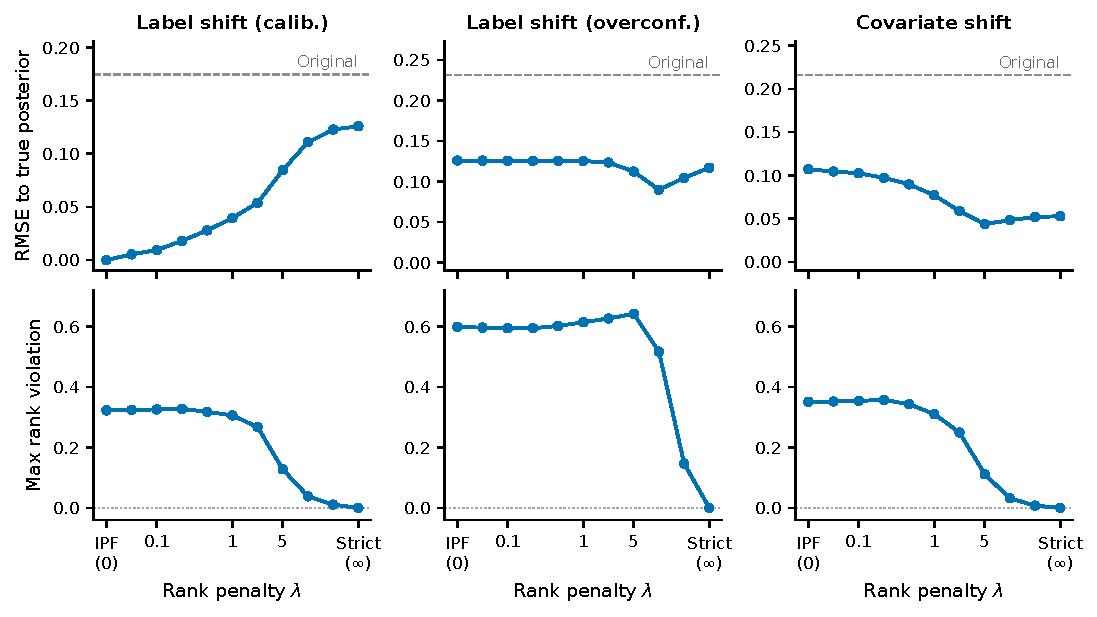
\includegraphics[width=\linewidth]{fig_synthetic_pareto.pdf}
\caption{Synthetic $\lambda$-path (means over 10 seeds) as the rank penalty $\lambda$ moves from $0$ (IPF) to $\infty$ (strict weak-order KL). Top row: RMSE to the exact target Bayes posterior (dashed line marks unadjusted probabilities). Bottom row: maximum weak-order rank violation. Under calibrated pure label shift (left), IPF is exact and raising $\lambda$ trades off accuracy. Under overconfidence (middle) and covariate shift (right), raising $\lambda$ reduces both posterior error and rank violations.}
\label{fig:synthetic}
\end{figure}

Table~\ref{tab:synthetic} and Figure~\ref{fig:synthetic} verify every part of Propositions~\ref{prop:ipf}--\ref{prop:pareto}. Under calibrated pure label shift, IPF achieves exact zero RMSE to truth (\SynPureIpfRmse{}) with \SynPureIpfRank{}\% rank preservation; strict weak-order KL raises rank preservation to \SynPureKlWeakRank{}\% at an RMSE cost of \SynPureKlWeakRmse{}, while soft KL ($\lambda=\SoftLam$) stays much closer (\SynPureKlSoftRmse{}). Once the pure-label-shift ideal breaks, the frontier flips. Under an overconfident source model, strict weak-order KL cuts RMSE to the true posterior below IPF (\SynOverKlWeakRmse{} versus \SynOverIpfRmse{}) and Brier score from \SynOverIpfBrier{} to \SynOverKlWeakBrier{} with zero rank violation. Under covariate shift, strict weak-order KL cuts posterior RMSE in half (\SynCovKlWeakRmse{} versus \SynCovIpfRmse{}) and soft KL achieves \SynCovKlSoftRmse{}. On the quantized tied inputs, exact weak-order block boundaries (\texttt{ties="weak"}) reduce KL divergence by an average of \TieKlDropPct\% relative to row-order tie constraints (\texttt{ties="stable"}). Meanwhile, Euclidean Dykstra failed to converge in 100\% of runs at $N=250$.

\subsection{Broad Real-Data Benchmark Across Six Datasets and Four Model Families}

To test whether these patterns hold outside synthetic mixtures, we evaluate \NumDatasets{} real multiclass datasets spanning $J=3$ to $10$ classes and diverse domains: Wine ($J=3$, chemistry), California Housing price quartiles ($J=4$, tabular; natural South-to-North California covariate shift), US Census CPS marital status ($J=4$, socioeconomic survey; natural Male-to-Female subpopulation shift), 20 Newsgroups political and religious discussion ($J=4$, TF-IDF + SVD text; short-to-long post shift), Forest Cover Type ($J=7$, ecological; near-to-far roadway shift), and Handwritten Digits ($J=10$, image features with heavy discrete ties; PC1 shift).

On each dataset we train \NumModels{} classifiers with distinct calibration profiles---logistic regression (\texttt{LogReg}, roughly calibrated), random forests (\texttt{RF}, underconfident with heavy score ties), histogram gradient boosting (\texttt{HGB}, overconfident), and a two-layer neural network (\texttt{MLP}, strongly overconfident)---reserving 25\% of source training data to fit a scalar temperature parameter $\tau$ for temperature-scaled baselines. We evaluate two regimes over \NumRealSeeds{} random seeds each: \emph{pure label shift} (Dirichlet-shifted test class priors) and \emph{covariate / subpopulation shift} (natural domain splits where $P(X \mid Y)$ also changes). We compare seven methods: unadjusted probabilities (\texttt{Original}), exact Sinkhorn \texttt{IPF}, source temperature scaling followed by IPF (\texttt{Temp + IPF}), Euclidean Dykstra (\texttt{Euclidean RPC}), strict weak-order KL (\texttt{KL weak}), soft weak-order KL (\texttt{KL soft}, $\lambda=\SoftLam$), and anchor-reference-decoupled temperature scaling plus soft KL (\texttt{Temp + KL soft}, $R = P_{\mathrm{temp}}$, $A = P$). Because methods can differ in convergence rate, Table~\ref{tab:real_summary} reports \emph{matched-pair} Brier and NLL improvements over IPF ($\text{IPF} - \text{method}$, multiplied by 1,000, with 95\% paired bootstrap confidence intervals) over runs where both methods converged, eliminating survivorship bias.

\begin{table}[htbp]
\centering\scriptsize\setlength{\tabcolsep}{2pt}
\caption{Matched-pair real-data benchmark across \NumDatasets{} datasets, \NumModels{} model families, and \NumRealSeeds{} seeds (\NumTotalRealRuns{} runs). $\Delta$Brier and $\Delta$NLL equal $(\text{IPF} - \text{method}) \times 1{,}000$ on matched converged runs (positive favors the named method), with 95\% paired bootstrap intervals. KL soft uses $\lambda=\SoftLam$.}
\label{tab:real_summary}
\begin{tabular}{llrrrrrrr}
\toprule
 &  & Conv. (\%) & $\Delta$Brier ($\times 10^3$) & $\Delta$NLL ($\times 10^3$) & AUROC & Rank (\%) & Max viol. & Col err \\
\midrule
Label shift & Original & 100.0 & -100.1 [-112.5, -87.1] & -229.0 [-259.9, -198.9] & 0.9210 & 100.0 & 0.000 & 28.80 \\
 & IPF & 94.6 & 0.0 (ref) & 0.0 (ref) & 0.9220 & 95.6 & 0.459 & $<0.01$ \\
 & Temp + IPF & 87.5 & +19.5 [+16.3, +22.8] & +105.5 [+86.2, +125.3] & 0.9157 & 93.3 & 0.427 & $<0.01$ \\
 & Euclidean RPC & 17.1 & -5.5 [-9.7, -2.0] & -28.7 [-45.6, -15.7] & 0.9976 & 100.0 & 0.000 & $<0.01$ \\
 & KL weak (strict) & 97.9 & -70.3 [-84.4, -55.9] & -112.8 [-146.2, -78.7] & 0.9179 & 100.0 & 0.000 & $<0.01$ \\
 & KL soft & 97.1 & -1.2 [-3.2, +0.9] & +1.7 [-3.0, +7.3] & 0.9228 & 97.9 & 0.376 & $<0.01$ \\
 & Temp + KL soft & 99.2 & +13.1 [+9.4, +17.1] & +87.2 [+69.8, +107.5] & 0.9226 & 97.6 & 0.310 & $<0.01$ \\
Covariate shift & Original & 100.0 & -202.2 [-228.8, -175.6] & -1223.7 [-1478.9, -981.4] & 0.8255 & 100.0 & 0.000 & 55.10 \\
 & IPF & 100.0 & 0.0 (ref) & 0.0 (ref) & 0.8404 & 89.0 & 0.635 & $<0.01$ \\
 & Temp + IPF & 100.0 & +36.4 [+30.0, +42.7] & +173.6 [+108.6, +234.5] & 0.8410 & 87.6 & 0.543 & $<0.01$ \\
 & Euclidean RPC & 12.0 & +20.9 [-4.6, +52.0] & +64.3 [-49.8, +199.4] & 0.8379 & 100.0 & 0.000 & $<0.01$ \\
 & KL weak (strict) & 97.4 & -17.3 [-30.4, -5.3] & +92.5 [+45.8, +147.5] & 0.8199 & 100.0 & 0.000 & $<0.01$ \\
 & KL soft & 99.0 & +12.3 [+8.6, +16.3] & +56.7 [+41.5, +74.9] & 0.8382 & 91.4 & 0.572 & $<0.01$ \\
 & Temp + KL soft & 97.9 & +39.8 [+32.4, +47.5] & +140.8 [+57.5, +223.9] & 0.8399 & 91.7 & 0.423 & $<0.01$ \\
\bottomrule
\end{tabular}

\end{table}

\begin{figure}[htbp]
\centering
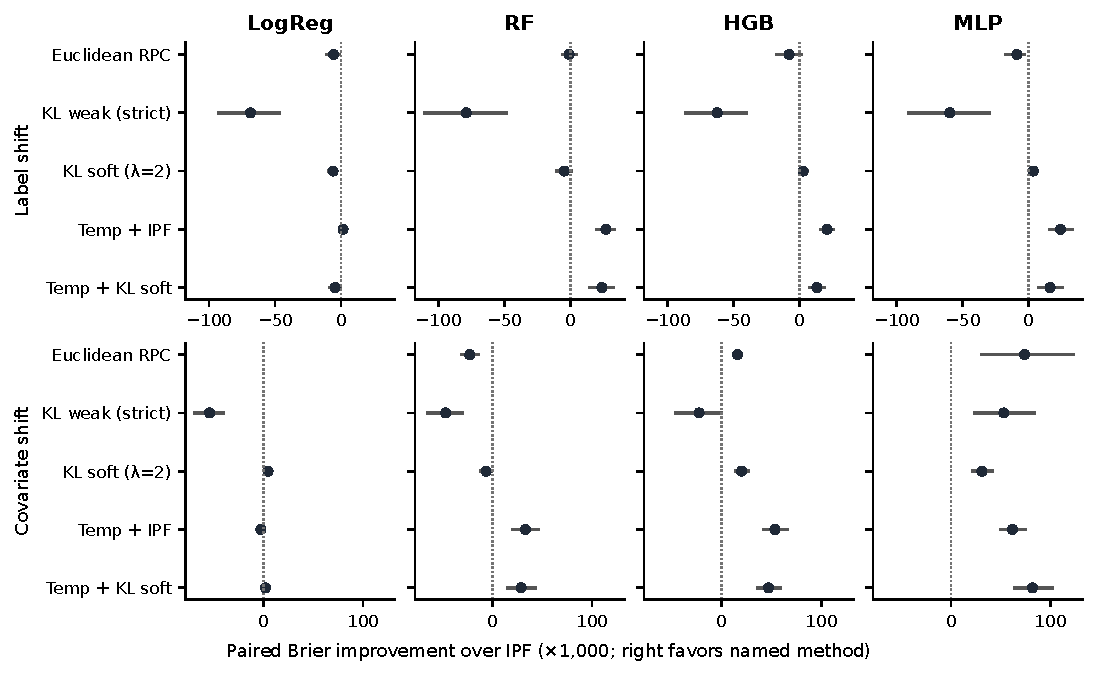
\includegraphics[width=\linewidth]{fig_real_brier_delta.pdf}
\caption{Matched-pair Brier improvement over IPF ($\times 1{,}000$; right favors the named method) by shift regime (rows) and model family (columns), with 95\% paired bootstrap confidence intervals over datasets and seeds. Euclidean RPC points reflect only the \RealEucConvPct\% of runs where Dykstra converged.}
\label{fig:real_brier}
\end{figure}

Table~\ref{tab:real_summary} and Figure~\ref{fig:real_brier} establish four empirical conclusions:
\begin{enumerate}[leftmargin=*,itemsep=2pt]
\item \textbf{KL geometry solves the convergence problem that breaks Euclidean projection.} Across all \NumTotalRealRuns{} real runs, Euclidean Dykstra converged on only \RealEucConvPct\% of problems (\DigitsEucConvPct\% on 10-class Digits). Exact weak-order KL converged on \RealKlWeakConvPct\%, soft KL on \RealKlSoftConvPct\%, and \texttt{Temp + KL soft} on \RealTempKlSoftConvPct\% (\DigitsKlSoftConvPct\% on Digits), matching exact column totals ($<0.01$ error).
\item \textbf{Pure label shift confirms the theoretical tradeoff.} Strict weak-order KL enforces \LabKlWeakRank{}\% rank preservation (zero violations) at a real matched-pair Brier penalty of \LabKlWeakDBrier{}$\times 10^{-3}$ (95\% CI [\LabKlWeakDBrierLo{}, \LabKlWeakDBrierHi{}]) versus IPF. Soft KL ($\lambda=\SoftLam$) nearly eliminates that cost (\LabKlSoftDBrier{}$\times 10^{-3}$, CI [\LabKlSoftDBrierLo{}, \LabKlSoftDBrierHi{}]; $\Delta\text{NLL} = \LabKlSoftDNll{}\times 10^{-3}$) while lifting rank preservation by \LabKlSoftDRank{} percentage points (\LabIpfRank{}\% to \LabKlSoftRank{}\%) and preserving macro one-vs-rest AUROC (\LabKlSoftAuroc{} versus \LabIpfAuroc{}).
\item \textbf{Temperature scaling before IPF worsens rank reversals, whereas decoupling fixes both.} \texttt{Temp + IPF} improves Brier (\LabTempIpfDBrier{} under label shift; \CovTempIpfDBrier{} under covariate shift) but \emph{reduces} rank preservation below plain IPF (\LabTempIpfDRank{} and \CovTempIpfDRank{} percentage points). Using temperature-scaled probabilities as the KL reference while anchoring ranks to $P$ (\texttt{Temp + KL soft}) reverses that loss, gaining \CovTempKlSoftDRank{} percentage points over IPF under covariate shift (a 3.8-point swing over \texttt{Temp + IPF}) while achieving the \emph{best} matched-pair Brier improvement of any method (\CovTempKlSoftDBrier{}$\times 10^{-3}$, CI [\CovTempKlSoftDBrierLo{}, \CovTempKlSoftDBrierHi{}]).
\item \textbf{Under covariate shift and overconfident models, rank regularization acts as a free regularizer.} Without any validation split for temperature scaling, \texttt{KL soft} beats IPF on Brier (\CovKlSoftDBrier{}$\times 10^{-3}$, CI [\CovKlSoftDBrierLo{}, \CovKlSoftDBrierHi{}]), NLL (\CovKlSoftDNll{}$\times 10^{-3}$), and rank preservation (\CovKlSoftDRank{} pp) simultaneously. Even strict \texttt{KL weak} improves NLL by \CovKlWeakDNll{}$\times 10^{-3}$ over IPF while achieving zero rank violations. Figure~\ref{fig:real_brier} shows this gain is concentrated in overconfident nonlinear classifiers (\texttt{HGB} and \texttt{MLP}): on those two models under covariate shift, \texttt{Temp + KL soft} improves mean Brier from \CovOverIpfBrier{} (IPF) and \CovOverTempIpfBrier{} (\texttt{Temp + IPF}) down to \CovOverTempKlSoftBrier{}, while raising rank preservation from \CovOverTempIpfRank{}\% to \CovOverTempKlSoftRank{}\%.
\end{enumerate}

\subsection{Survey Marginal Calibration: US Census CPS Subpopulation Shift}

To examine \citet{mitchell2025}'s survey-statistics motivation directly, we inspect the US Census CPS four-class marital-status task in detail: each classifier is trained on male respondents and calibrated to match known female marginal counts ($N=250$ per batch, \NumRealSeeds{} seeds). Table~\ref{tab:census} reports results by model family, and Figure~\ref{fig:real_pareto} plots the full $\lambda$-Pareto frontier alongside California Housing under covariate versus pure label shift.

\begin{table}[htbp]
\centering\footnotesize\setlength{\tabcolsep}{4pt}
\caption{US Census CPS subpopulation shift (Male $\to$ Female, 4-class marital status, \NumRealSeeds{} seeds). Euclidean RPC failed to converge in 100\% of runs (``--''); KL soft uses $\lambda=\SoftLam$.}
\label{tab:census}
\begin{tabular}{llrrrrrrr}
\toprule
 &  & Brier & NLL & ECE & AUROC & Rank rate & Max viol. & Col err \\
\midrule
LogReg & Original & 0.6840 & 1.3092 & 0.2177 & 0.7771 & 1.0000 & 0.000 & 70.08 \\
 & IPF & 0.5286 & 1.0169 & 0.0762 & 0.7797 & 0.9387 & 0.250 & $<0.01$ \\
 & Temp + IPF & 0.5291 & 1.0153 & 0.0784 & 0.7795 & 0.9383 & 0.243 & $<0.01$ \\
 & Euclidean RPC & -- & -- & -- & -- & -- & -- & -- \\
 & KL weak (strict) & 0.5799 & 1.1158 & 0.1145 & 0.7764 & 1.0000 & 0.000 & $<0.01$ \\
 & KL soft & 0.5359 & 1.0384 & 0.0814 & 0.7789 & 0.9798 & 0.217 & $<0.01$ \\
 & Temp + KL soft & 0.5369 & 1.0375 & 0.0739 & 0.7788 & 0.9804 & 0.203 & $<0.01$ \\
RF & Original & 0.6978 & 1.5976 & 0.2233 & 0.7483 & 1.0000 & 0.000 & 66.28 \\
 & IPF & 0.5799 & 1.2980 & 0.1255 & 0.7505 & 0.9392 & 0.465 & $<0.01$ \\
 & Temp + IPF & 0.5570 & 1.1111 & 0.0626 & 0.7474 & 0.9178 & 0.370 & $<0.01$ \\
 & Euclidean RPC & -- & -- & -- & -- & -- & -- & -- \\
 & KL weak (strict) & 0.5823 & 1.1397 & 0.1053 & 0.7486 & 1.0000 & 0.000 & $<0.01$ \\
 & KL soft & 0.5656 & 1.2513 & 0.0960 & 0.7509 & 0.9663 & 0.490 & $<0.01$ \\
 & Temp + KL soft & 0.5607 & 1.0954 & 0.0801 & 0.7438 & 0.9654 & 0.405 & $<0.01$ \\
HGB & Original & 0.7101 & 1.5539 & 0.2613 & 0.7683 & 1.0000 & 0.000 & 69.38 \\
 & IPF & 0.5703 & 1.1702 & 0.1578 & 0.7731 & 0.9342 & 0.550 & $<0.01$ \\
 & Temp + IPF & 0.5324 & 1.0141 & 0.0754 & 0.7736 & 0.9310 & 0.391 & $<0.01$ \\
 & Euclidean RPC & -- & -- & -- & -- & -- & -- & -- \\
 & KL weak (strict) & 0.5758 & 1.1659 & 0.1148 & 0.7653 & 1.0000 & 0.000 & $<0.01$ \\
 & KL soft & 0.5481 & 1.1279 & 0.1257 & 0.7719 & 0.9622 & 0.559 & $<0.01$ \\
 & Temp + KL soft & 0.5302 & 1.0237 & 0.0764 & 0.7722 & 0.9702 & 0.348 & $<0.01$ \\
MLP & Original & 0.7452 & 1.9837 & 0.2896 & 0.7214 & 1.0000 & 0.000 & 65.23 \\
 & IPF & 0.6453 & 1.5856 & 0.2165 & 0.7242 & 0.9353 & 0.630 & $<0.01$ \\
 & Temp + IPF & 0.5733 & 1.1313 & 0.0801 & 0.7250 & 0.9257 & 0.401 & $<0.01$ \\
 & Euclidean RPC & -- & -- & -- & -- & -- & -- & -- \\
 & KL weak (strict) & 0.5885 & 1.2024 & 0.1132 & 0.7208 & 1.0000 & 0.000 & $<0.01$ \\
 & KL soft & 0.6186 & 1.5043 & 0.1731 & 0.7231 & 0.9551 & 0.662 & $<0.01$ \\
 & Temp + KL soft & 0.5696 & 1.1204 & 0.0809 & 0.7225 & 0.9666 & 0.365 & $<0.01$ \\
\bottomrule
\end{tabular}

\end{table}

\begin{figure}[htbp]
\centering
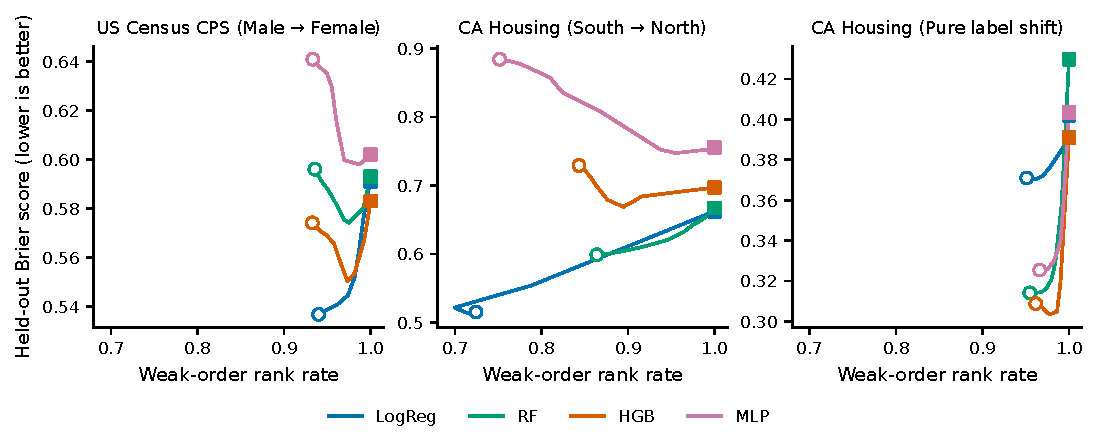
\includegraphics[width=\linewidth]{fig_real_pareto.pdf}
\caption{Held-out Brier score versus weak-order rank preservation rate along the KL $\lambda$-path (means over 5 seeds). Open circles mark IPF ($\lambda=0$); filled squares mark strict weak-order KL ($\lambda=\infty$). Under real subpopulation and geographic covariate shifts (left and middle), moderate rank regularization lowers Brier score for nonlinear classifiers (MLP, HGB, RF) while raising rank preservation; under pure label shift (right) and calibrated LogReg, the curve slopes upward as Proposition~\ref{prop:ipf} predicts.}
\label{fig:real_pareto}
\end{figure}

The US Census application shows both sides of the story clearly. On a well-calibrated linear model (\texttt{LogReg}), IPF achieves Brier \CenLrIpfBrier{} at \CenLrIpfRank{}\% rank preservation, and soft KL trades a small Brier increment (\CenLrKlSoftBrier{}) to reach \CenLrKlSoftRank{}\% rank preservation. On an overconfident neural network (\texttt{MLP}), IPF suffers Brier \CenMlpIpfBrier{} and NLL \CenMlpIpfNll{} with \CenMlpIpfRank{}\% rank preservation; strict \texttt{KL weak} alone---using zero validation labels---drops Brier to \CenMlpKlWeakBrier{} and NLL to \CenMlpKlWeakNll{} at \CenMlpKlWeakRank{}\% rank preservation, and \texttt{Temp + KL soft} achieves the best overall accuracy (Brier \CenMlpTempKlSoftBrier{}, NLL \CenMlpTempKlSoftNll{}, Rank \CenMlpTempKlSoftRank{}\%), beating \texttt{Temp + IPF} (Brier \CenMlpTempIpfBrier{}, NLL \CenMlpTempIpfNll{}, Rank \CenMlpTempIpfRank{}\%) on every metric simultaneously. On \texttt{HGB}, \texttt{Temp + KL soft} likewise beats \texttt{Temp + IPF} on Brier (\CenHgbTempKlSoftBrier{} versus \CenHgbTempIpfBrier{}) while raising rank preservation from \CenHgbTempIpfRank{}\% to \CenHgbTempKlSoftRank{}\%.

\section{Practical Guidance and Limitations}

The theory and \NumTotalRealRuns{}-run benchmark yield a clear decision rule for practitioners matching multiclass probabilities to known aggregate totals:
\begin{enumerate}[leftmargin=*,itemsep=2pt]
\item \textbf{Use KL geometry, never Euclidean Dykstra.} Additive Euclidean updates distort probabilities near zero and fail to converge on most realistic problems (\RealEucConvPct\% convergence).
\item \textbf{Use exact weak-order tie handling (\texttt{ties="weak"}).} Whenever predictions come from trees, rounded scores, or discrete models, block-boundary constraints avoid artificial intra-tie distortions and strictly lower KL divergence.
\item \textbf{Match the penalty $\lambda$ to the shift regime and governance requirement.} Under known pure label shift with a well-calibrated linear model and no ranking constraint, standard IPF is Bayes-optimal. Whenever a nonlinear model is deployed under covariate or subpopulation shift, or when within-class rankings matter, use \texttt{Temp + KL soft} (if a source validation split is available) or \texttt{KL soft} ($\lambda \approx 1\text{--}2$); reserve strict \texttt{KL weak} for settings with hard institutional no-reversal rules.
\end{enumerate}

Three limitations bound these findings. First, all methods operate at the batch level for a given matrix $P \in \mathbb{R}^{N \times J}$ and known target totals $T$; estimating uncertain totals $\hat{T}$ from noisy auxiliary surveys adds sampling variance not modeled here. Second, solving the exponential-cone program scales roughly super-linearly in $NJ$: batches of $N=200\text{--}400$ with $J \le 10$ solve in $0.1\text{--}3$ seconds, whereas tens of thousands of rows require stratified batching or first-order splitting. Third, soft KL introduces a penalty parameter $\lambda$; while the untuned default $\lambda=\SoftLam$ performed robustly across all \NumDatasets{} datasets and \NumModels{} model families, exploring the $\lambda$-Pareto frontier via \texttt{calibrate\_kl\_pareto} remains good practice in high-stakes deployments.

{\small
\bibliographystyle{working-paper-apsr}
\bibliography{multiclass}
}

\clearpage
\appendix

\section{Proofs and Conic Formulation}
\label{app:proofs}

\subsection{Proof of \texorpdfstring{Proposition~\ref{prop:ipf}}{Proposition 1}}

\begin{proof}
Write $Z_i = \sum_{k=1}^J b_k P_{ik} > 0$, so $Q^{\mathrm{IPF}}_{ij} = b_j P_{ij} / Z_i$.

\emph{(a) Binary preservation.} For $J=2$, $P_{i2} = 1 - P_{i1}$, so
\[
Q^{\mathrm{IPF}}_{i1} = \frac{b_1 P_{i1}}{b_1 P_{i1} + b_2(1 - P_{i1})} = \frac{1}{1 + (b_2/b_1)(P_{i1}^{-1} - 1)},
\]
which is strictly increasing in $P_{i1}$ since $b_1, b_2 > 0$. The same holds for $Q^{\mathrm{IPF}}_{i2} = 1 - Q^{\mathrm{IPF}}_{i1}$.

\emph{(b) Pairwise odds-ratio invariance.} For any $j, k$, the denominator $Z_i$ cancels:
\[
\frac{Q^{\mathrm{IPF}}_{i j}}{Q^{\mathrm{IPF}}_{i k}} = \frac{b_j}{b_k}\,\frac{P_{ij}}{P_{ik}}.
\]
Since $b_j / b_k > 0$, the ratio $Q^{\mathrm{IPF}}_{ij} / Q^{\mathrm{IPF}}_{ik}$ is a strictly increasing linear function of $P_{ij} / P_{ik}$.

\emph{(c) Exact reversal condition.} Suppose $P_{i_1 j} > P_{i_2 j} > 0$. Then
\[
Q^{\mathrm{IPF}}_{i_1 j} < Q^{\mathrm{IPF}}_{i_2 j}
\;\Longleftrightarrow\;
\frac{b_j P_{i_1 j}}{Z_{i_1}} < \frac{b_j P_{i_2 j}}{Z_{i_2}}
\;\Longleftrightarrow\;
\frac{Z_{i_1}}{Z_{i_2}} > \frac{P_{i_1 j}}{P_{i_2 j}}.
\]
If $b_k = b_j$ for all $k \ne j$, then $Z_i = b_j \sum_k P_{ik} = b_j$, so $Z_{i_1}/Z_{i_2} = 1 < P_{i_1 j}/P_{i_2 j}$ and no reversal occurs. Similarly, if $P_{i_1 k} = P_{i_2 k}$ for all $k \ne j$, then $P_{i_1 j} = 1 - \sum_{k \ne j} P_{i_1 k} = P_{i_2 j}$, contradicting $P_{i_1 j} > P_{i_2 j}$. Hence some third class $k \ne j$ with $b_k \ne b_j$ and $P_{i_1 k} \ne P_{i_2 k}$ is necessary.

\emph{(d) Pure-label-shift impossibility.} Under $P_{\mathrm{tgt}}(X \mid Y) = P_{\mathrm{src}}(X \mid Y)$, Bayes' rule gives
\[
P_{\mathrm{tgt}}(Y=j \mid X_i) = \frac{(\pi^{\mathrm{tgt}}_j / \pi^{\mathrm{src}}_j)\, P_{\mathrm{src}}(Y=j \mid X_i)}{\sum_k (\pi^{\mathrm{tgt}}_k / \pi^{\mathrm{src}}_k)\, P_{\mathrm{src}}(Y=k \mid X_i)}.
\]
This matrix lies in $\mathcal{C}(T)$ for $T_j = \sum_i P_{\mathrm{tgt}}(Y=j \mid X_i)$ and has the multiplicative form~\eqref{eq:ipf}. By uniqueness of the KL projection onto $\mathcal{C}(T)$, it equals $Q^{\mathrm{IPF}}$. Whenever condition~(c) holds, the unique Bayes-optimal matrix in $\mathcal{C}(T)$ violates~\eqref{eq:weak_order}, so no matrix can satisfy all three properties simultaneously.
\end{proof}

\subsection{Proof of \texorpdfstring{Proposition~\ref{prop:ties}}{Proposition 2}}

\begin{proof}
($\Leftarrow$) Suppose $u_{j,1} \le \cdots \le u_{j,K_j-1}$ satisfy~\eqref{eq:boundaries}. Take any $i_1, i_2$ with $A_{i_1 j} < A_{i_2 j}$, so $i_1 \in B_{j,k}$ and $i_2 \in B_{j,k'}$ with $k < k'$. Then $Q_{i_1 j} \le u_{j,k} \le u_{j,k'-1} \le Q_{i_2 j}$.

($\Rightarrow$) Conversely, suppose $Q_{\cdot j}$ satisfies~\eqref{eq:weak_order}. For $k = 1,\dots,K_j - 1$, set $u_{j,k} = \max_{r \le k} \max_{i \in B_{j,r}} Q_{ij}$. By construction $u_{j,1} \le \cdots \le u_{j,K_j-1}$ and $Q_{ij} \le u_{j,k}$ for all $i \in B_{j,k}$ ($k < K_j$). For any $i' \in B_{j,k'}$ with $k' > 1$ and any $i \in B_{j,r}$ with $r \le k' - 1$, we have $A_{ij} < A_{i'j}$, so~\eqref{eq:weak_order} gives $Q_{ij} \le Q_{i'j}$. Taking the maximum over $r \le k'-1$ and $i \in B_{j,r}$ yields $u_{j,k'-1} \le Q_{i'j}$.

Each unit $i \in B_{j,k}$ participates in at most two inequalities ($Q_{ij} \le u_{j,k}$ and $u_{j,k-1} \le Q_{ij}$), plus $K_j - 2$ ordering inequalities among $u$, totaling at most $2N + K_j - 2$ linear inequalities. Because blocks $B_{j,k}$ depend only on the values of $A_{\cdot j}$ and not on row indices, $\mathcal{W}(A)$ is invariant to row permutations. Every matrix in the stable-sort cone $\mathcal{S}(A)$ trivially satisfies~\eqref{eq:weak_order}, so $\mathcal{S}(A) \subseteq \mathcal{W}(A)$, giving the divergence inequality. Finally, $Q_{ij} = T_j/N$ lies in $\mathcal{C}(T)$ and satisfies~\eqref{eq:weak_order} with $u_{j,k} = T_j/N$.
\end{proof}

\subsection{Proofs of \texorpdfstring{Propositions~\ref{prop:bregman} and~\ref{prop:pareto}}{Propositions 3 and 4}}

\begin{proof}[Proof of Proposition~\ref{prop:bregman}]
Form the Lagrangian for~\eqref{eq:soft} with multipliers $\nu \in \mathbb{R}^N$ on $Q\mathbf{1}_J = \mathbf{1}_N$, $\mu \in \mathbb{R}^J$ on $Q^\top\mathbf{1}_N = T$, and $\alpha_r \ge 0$ on each relaxed inequality $s_r^\top (q, u) - v_r \le 0$. Stationarity with respect to $v_r \ge 0$ gives $0 \le \alpha_r \le \lambda$. Stationarity with respect to $Q_{ij} > 0$ yields
\[
\phi'(Q^\star_{ij}) - \phi'(R_{ij}) + \nu_i + \mu_j + \gamma_{ij} = 0,
\]
where $\gamma_{ij}$ is the signed sum of active multipliers $\alpha_r$ incident to $Q_{ij}$. Substituting $\phi'(x) = \log x$ gives $Q^\star_{ij} = R_{ij}\exp(-\nu_i - \mu_j - \gamma_{ij})$, which is strictly positive when $R_{ij} > 0$ and reduces to~\eqref{eq:ipf} with $b_j = e^{-\mu_j}$ when $\lambda = 0$ ($\alpha_r = 0$). Substituting $\phi'(x) = x$ with nonnegativity multipliers $\eta_{ij} \ge 0$ yields $Q^\star_{ij} = \max(0, R_{ij} - \nu_i - \mu_j - \gamma_{ij})$.
\end{proof}

\begin{proof}[Proof of Proposition~\ref{prop:pareto}]
Write $\operatorname{KL}(Q \| R) = \sum_{i,j: R_{ij} > 0} Q_{ij}\log Q_{ij} - \sum_{i,j: R_{ij} > 0} Q_{ij}\log R_{ij}$ (dropping constants since $\sum_{i,j} Q_{ij} = N$). Introducing one epigraph variable $t_{ij}$ per positive entry $R_{ij} > 0$ with $t_{ij} \ge Q_{ij}\log Q_{ij}$ is equivalent to the exponential-cone constraint $(-t_{ij}, Q_{ij}, 1) \in \mathcal{K}_{\exp} = \{(x,y,z) : y > 0,\; z \ge y\exp(x/y)\} \cup \{(x,0,z) : x \le 0, z \ge 0\}$. Combining with the linear equalities of $\mathcal{C}(T)$ and linear inequalities~\eqref{eq:boundaries} yields a convex exponential-cone program of size $O(NJ)$ solved directly by Clarabel \citep{goulart2024clarabel}.

For monotonicity, let $0 \le \lambda_1 < \lambda_2$ with optima $Q_1 = Q^\star(\lambda_1)$ and $Q_2 = Q^\star(\lambda_2)$. Optimality gives
\begin{align*}
\operatorname{KL}(Q_1 \| R) + \lambda_1 V_A(Q_1) &\le \operatorname{KL}(Q_2 \| R) + \lambda_1 V_A(Q_2), \\
\operatorname{KL}(Q_2 \| R) + \lambda_2 V_A(Q_2) &\le \operatorname{KL}(Q_1 \| R) + \lambda_2 V_A(Q_1).
\end{align*}
Adding the two inequalities yields $(\lambda_2 - \lambda_1)[V_A(Q_2) - V_A(Q_1)] \le 0$, so $V_A(Q_2) \le V_A(Q_1)$. Substituting back into the first inequality gives $\operatorname{KL}(Q_1 \| R) \le \operatorname{KL}(Q_2 \| R)$.
\end{proof}

\clearpage
\section{Complete Real-Data Results and Reproduction}
\label{app:details}

Table~\ref{tab:real_by_dataset} reports mean performance for every dataset and shift regime averaged across all four model families and ten seeds.

\begingroup\footnotesize\setlength{\tabcolsep}{4pt}
\begin{longtable}{llrrrrrr}
\caption{Mean real-data benchmark performance by dataset and shift regime (averaged across four model families and ten seeds; converged solves only; KL soft uses $\lambda=2$). ``--'' indicates zero converged solves.} \label{tab:real_by_dataset} \\
\toprule
 &  & Brier & NLL & AUROC & Rank rate & Max viol. & Conv. (\%) \\
\midrule
\endfirsthead
\caption[]{Mean real-data benchmark performance by dataset and shift regime (averaged across four model families and ten seeds; converged solves only; KL soft uses $\lambda=2$). ``--'' indicates zero converged solves.} \\
\toprule
 &  & Brier & NLL & AUROC & Rank rate & Max viol. & Conv. (\%) \\
\midrule
\endhead
\midrule
\multicolumn{8}{r}{Continued on next page} \\
\midrule
\endfoot
\bottomrule
\endlastfoot
Wine (J=3) (Label) & IPF & 0.0301 & 0.0645 & 0.9993 & 0.9747 & 0.090 & 90 \\
 & Temp + IPF & 0.0267 & 0.0522 & 0.9988 & 0.9688 & 0.133 & 38 \\
 & Euclidean RPC & 0.0335 & 0.0808 & 0.9991 & 1.0000 & 0.000 & 100 \\
 & KL weak (strict) & 0.0283 & 0.0604 & 0.9991 & 1.0000 & 0.000 & 100 \\
 & KL soft & 0.0276 & 0.0589 & 0.9992 & 0.9945 & 0.014 & 98 \\
 & Temp + KL soft & 0.0165 & 0.0347 & 0.9993 & 0.9950 & 0.046 & 98 \\
CA Housing (J=4) (Label) & IPF & 0.3128 & 0.6004 & 0.8830 & 0.9582 & 0.397 & 100 \\
 & Temp + IPF & 0.3018 & 0.5593 & 0.8830 & 0.9552 & 0.355 & 100 \\
 & Euclidean RPC & -- & -- & -- & -- & -- & 0 \\
 & KL weak (strict) & 0.3980 & 0.7696 & 0.8735 & 1.0000 & 0.000 & 100 \\
 & KL soft & 0.3249 & 0.6289 & 0.8769 & 0.9833 & 0.326 & 98 \\
 & Temp + KL soft & 0.3116 & 0.5839 & 0.8769 & 0.9835 & 0.267 & 100 \\
US Census CPS (J=4) (Label) & IPF & 0.4951 & 1.0798 & 0.7720 & 0.9176 & 0.574 & 100 \\
 & Temp + IPF & 0.4661 & 0.8795 & 0.7711 & 0.9089 & 0.440 & 100 \\
 & Euclidean RPC & -- & -- & -- & -- & -- & 0 \\
 & KL weak (strict) & 0.5108 & 0.9762 & 0.7573 & 1.0000 & 0.000 & 100 \\
 & KL soft & 0.4874 & 1.0411 & 0.7652 & 0.9566 & 0.519 & 100 \\
 & Temp + KL soft & 0.4753 & 0.8836 & 0.7621 & 0.9665 & 0.312 & 100 \\
20 Newsgroups (J=4) (Label) & IPF & 0.2535 & 0.5887 & 0.9448 & 0.9650 & 0.565 & 100 \\
 & Temp + IPF & 0.2265 & 0.4238 & 0.9454 & 0.9385 & 0.440 & 100 \\
 & Euclidean RPC & 0.2648 & 0.9097 & 0.9387 & 1.0000 & 0.000 & 2 \\
 & KL weak (strict) & 0.3233 & 0.6837 & 0.9393 & 1.0000 & 0.000 & 100 \\
 & KL soft & 0.2557 & 0.5947 & 0.9436 & 0.9818 & 0.526 & 95 \\
 & Temp + KL soft & 0.2342 & 0.4410 & 0.9435 & 0.9780 & 0.387 & 98 \\
Forest Cover (J=7) (Label) & IPF & 0.2710 & 0.5447 & 0.9586 & 0.9657 & 0.703 & 100 \\
 & Temp + IPF & 0.2563 & 0.4666 & 0.9590 & 0.9126 & 0.608 & 100 \\
 & Euclidean RPC & -- & -- & -- & -- & -- & 0 \\
 & KL weak (strict) & 0.4861 & 0.9880 & 0.9492 & 1.0000 & 0.000 & 100 \\
 & KL soft & 0.2786 & 0.5485 & 0.9569 & 0.9756 & 0.656 & 92 \\
 & Temp + KL soft & 0.2677 & 0.4906 & 0.9564 & 0.9585 & 0.553 & 100 \\
Digits (J=10) (Label) & IPF & 0.0456 & 0.1178 & 0.9995 & 0.9594 & 0.364 & 78 \\
 & Temp + IPF & 0.0223 & 0.0515 & 0.9996 & 0.9354 & 0.396 & 88 \\
 & Euclidean RPC & -- & -- & -- & -- & -- & 0 \\
 & KL weak (strict) & 0.0539 & 0.1500 & 0.9993 & 1.0000 & 0.000 & 88 \\
 & KL soft & 0.0378 & 0.0962 & 0.9995 & 0.9809 & 0.232 & 100 \\
 & Temp + KL soft & 0.0216 & 0.0491 & 0.9996 & 0.9769 & 0.289 & 100 \\
CA Housing (J=4) (Cov.) & IPF & 0.6931 & 1.5106 & 0.7021 & 0.7942 & 0.831 & 100 \\
 & Temp + IPF & 0.6547 & 1.2905 & 0.7024 & 0.7997 & 0.757 & 100 \\
 & Euclidean RPC & 0.7264 & 1.6002 & 0.5233 & 1.0000 & 0.000 & 12 \\
 & KL weak (strict) & 0.6931 & 1.3731 & 0.6401 & 1.0000 & 0.000 & 100 \\
 & KL soft & 0.6668 & 1.4074 & 0.6930 & 0.8541 & 0.694 & 100 \\
 & Temp + KL soft & 0.6412 & 1.2510 & 0.6887 & 0.8767 & 0.479 & 95 \\
US Census CPS (J=4) (Cov.) & IPF & 0.5810 & 1.2677 & 0.7569 & 0.9368 & 0.474 & 100 \\
 & Temp + IPF & 0.5479 & 1.0680 & 0.7563 & 0.9282 & 0.351 & 100 \\
 & Euclidean RPC & -- & -- & -- & -- & -- & 0 \\
 & KL weak (strict) & 0.5816 & 1.1559 & 0.7528 & 1.0000 & 0.000 & 100 \\
 & KL soft & 0.5671 & 1.2305 & 0.7562 & 0.9659 & 0.482 & 100 \\
 & Temp + KL soft & 0.5491 & 1.0686 & 0.7546 & 0.9708 & 0.328 & 98 \\
20 Newsgroups (J=4) (Cov.) & IPF & 0.2284 & 0.5615 & 0.9728 & 0.9774 & 0.362 & 100 \\
 & Temp + IPF & 0.1911 & 0.3766 & 0.9733 & 0.9383 & 0.209 & 100 \\
 & Euclidean RPC & 0.2648 & 0.7491 & 0.9654 & 1.0000 & 0.000 & 22 \\
 & KL weak (strict) & 0.2308 & 0.5938 & 0.9722 & 1.0000 & 0.000 & 100 \\
 & KL soft & 0.2261 & 0.5653 & 0.9730 & 0.9844 & 0.315 & 98 \\
 & Temp + KL soft & 0.1960 & 0.3902 & 0.9730 & 0.9874 & 0.136 & 100 \\
Forest Cover (J=7) (Cov.) & IPF & 0.6447 & 1.6831 & 0.8811 & 0.8973 & 0.706 & 100 \\
 & Temp + IPF & 0.5914 & 1.2113 & 0.8830 & 0.8627 & 0.582 & 100 \\
 & Euclidean RPC & 0.5784 & 1.2067 & 0.8852 & 1.0000 & 0.000 & 22 \\
 & KL weak (strict) & 0.6219 & 1.4481 & 0.8690 & 1.0000 & 0.000 & 100 \\
 & KL soft & 0.6337 & 1.6228 & 0.8819 & 0.9078 & 0.650 & 98 \\
 & Temp + KL soft & 0.5864 & 1.2148 & 0.8824 & 0.8844 & 0.473 & 98 \\
Digits (J=10) (Cov.) & IPF & 0.5544 & 1.5254 & 0.9013 & 0.8329 & 0.846 & 100 \\
 & Temp + IPF & 0.5386 & 1.8296 & 0.9024 & 0.8441 & 0.885 & 100 \\
 & Euclidean RPC & -- & -- & -- & -- & -- & 0 \\
 & KL weak (strict) & 0.7023 & 1.5658 & 0.8872 & 1.0000 & 0.000 & 84 \\
 & KL soft & 0.5410 & 1.4073 & 0.9049 & 0.8448 & 0.753 & 100 \\
 & Temp + KL soft & 0.5273 & 1.9895 & 0.9054 & 0.8503 & 0.772 & 100 \\
\end{longtable}

\endgroup

\subsection{Reproduction}

All package tests, benchmark experiments, exhibits, and this manuscript reproduce from the repository root (\url{https://github.com/finite-sample/rank-preserving-calibration}, v0.12.0):
\begin{lstlisting}
uv sync --all-groups
uv run pytest
uv run --with pandas --with matplotlib python ms/experiments/run_benchmark.py
uv run --with pandas --with matplotlib --with jinja2 python ms/experiments/build_exhibits.py
latexmk -cd -pdf -interaction=nonstopmode -halt-on-error -Werror ms/rank-preserving-multiclass.tex
\end{lstlisting}

\end{document}
